\section{Artificial Neural Networks}
The concept of \gls{ai} emerged in the mid-twentieth century as scientists aimed to design computational systems capable of reasoning in ways comparable to human cognition. The term was formally introduced by John McCarthy during the 1956 Dartmouth Conference, marking the official establishment of \gls{ai} as a scientific research field \cite{Zhang2023AI70Years}. Early \gls{ai} systems relied on symbolic reasoning, encoding expert knowledge in fixed logical rules; however, such methodologies proved inadequate when confronted with complex and heterogeneous data environments.

In the 1980s, the paradigm of \gls{ml} was proposed to address these limitations. This approach shifted focus from explicitly programmed rule-based models to data-driven methods capable of improving performance through experience \cite{Finley2024ClassicalML}. The pioneering work of Arthur Samuel demonstrated that computers could autonomously learn patterns from data rather than relying solely on predefined logic, laying the foundation for future development.

Around 2010, the field underwent a significant transformation with the emergence of \gls{dl}. This new paradigm utilized hierarchical, multi-layered neural networks capable of automatically extracting complex features from raw data, fundamentally changing fields like computer vision and natural language processing \cite{Azizov2024DecadeDL}. The extraordinary success of deep learning has been supported by advances in computational power, large-scale labeled datasets, and optimized training algorithms.

\subsection{Neural Network and Neuron Perceptron}
The foundational objective of \gls{ai} was to develop computational models that emulate the behavior of biological neurons. The perceptron, as one of the earliest such models, produces an output of $+1$ or $-1$ based on a weighted sum of its inputs, functioning as a linear classifier defined by \cite{Gabrie2023} \begin{equation}
h(\mathbf{x}) = \mathrm{sign}(\mathbf{w}^\top \mathbf{x}).
\end{equation} The perceptron algorithm seeks a weight vector $\mathbf{w}$ that defines a hyperplane separating data points from different classes, maximizing the margin between them. The figure \ref{fig:perceptron} shows how perceptron works. This approach assumes linear separability; otherwise, the algorithm may not converge. To address this, multiple perceptrons can be combined to form more complex, nonlinear functions.


Replacing the step function with a sigmoid activation leads to logistic regression, which models the probability of class membership and enables gradient-based optimization. By stacking layers of perceptrons, one obtains a multilayer perceptron or feed-forward neural network, which can approximate nonlinear functions and learn hierarchical representations \cite{Schmid2025}. The design of such networks aims to balance expressive power with generalization, mitigating overfitting by controlling model complexity and regularization \cite{NNWork2025}.

\begin{figure}[ht]
    \centering
    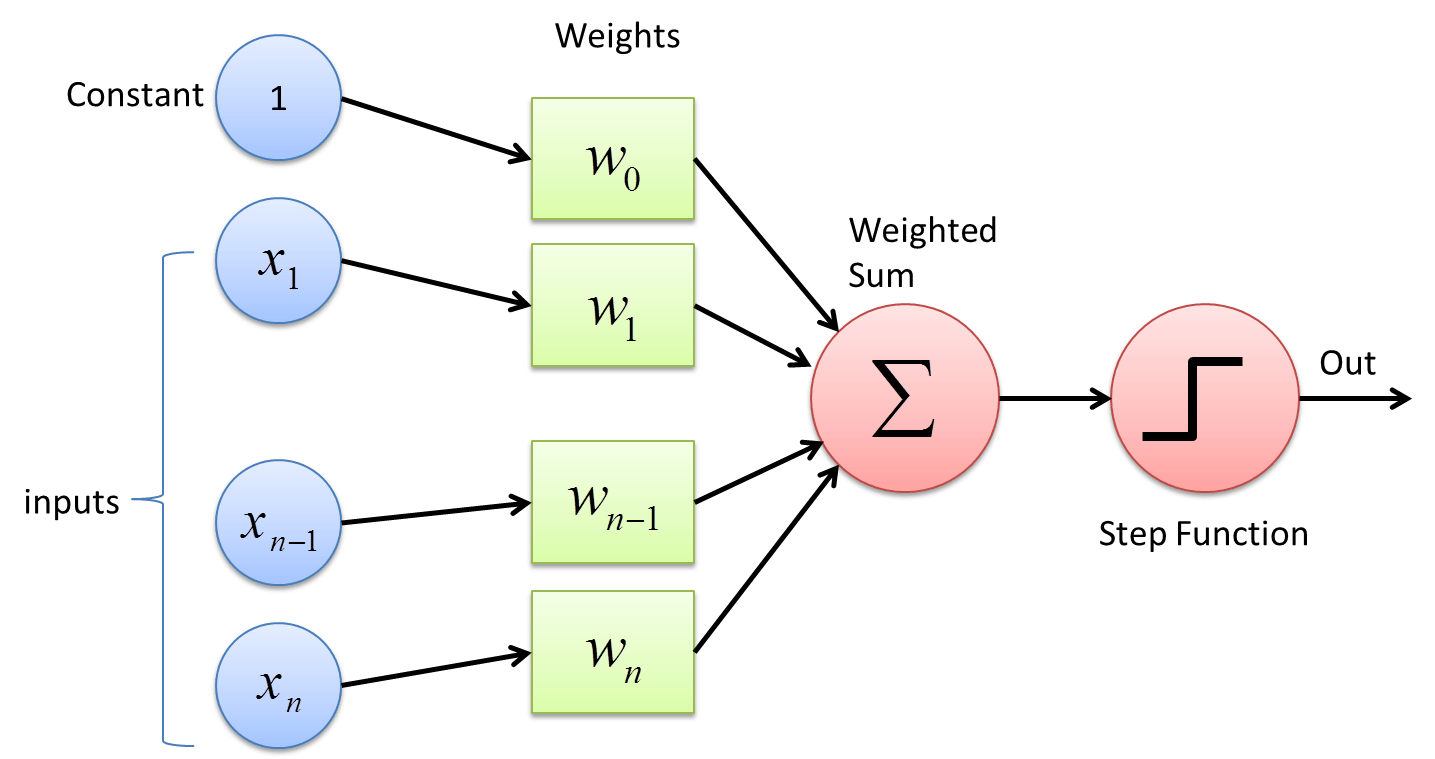
\includegraphics[width=0.80\textwidth]{chap2/figure/perceptron.png}
    \caption{Overview of a perceptron \cite{deepai_perceptron}.}
    \label{fig:perceptron}
\end{figure}




\subsection{Training Neural Network}
Training a neural network involves determining the set of weights $\boldsymbol{\theta}$ that minimize a loss function, which quantifies the discrepancy between predicted and actual values. For regression tasks, a common choice is the mean squared error:

\begin{equation}
\ell_{\theta} = \frac{1}{n} \sum_{i=1}^{n} (y_i - g_{\theta}(x_i))^2
\end{equation}

where $y_i$ is the true value, $g_{\theta}(x_i)$ is the network's prediction, and $n$ is the number of samples \cite{Gabrie2023}.

Since the loss function is generally non-convex for neural networks, it is typically minimized using the Gradient Descent algorithm. This iterative method updates the weights by moving in the direction of the negative gradient of the loss:

\begin{equation}
\theta^{(t+1)} = \theta^{(t)} - \alpha \nabla \ell_{\theta^{(t)}}
\end{equation}

Here, $\alpha > 0$ is the learning rate, a hyperparameter that controls the step size at each iteration. Choosing an appropriate learning rate is crucial: a value too large may cause the algorithm to overshoot minima, while a value too small can result in slow convergence.

For large datasets, computing the gradient over the entire dataset at each step is computationally expensive. To address this, Stochastic Gradient Descent (SGD) is used, where the gradient is estimated using a small batch of samples. After all batches are processed, one epoch is completed.

In feedforward neural networks, each neuron composes multiple functions, making gradient computation complex. To automate this, the concept of a computational graph is introduced: an acyclic graph representing the composition of functions computed by the network. This structure enables efficient calculation of derivatives via backpropagation, where gradients are computed from the output layer backward to the input, leveraging the chain rule, as shown in Figure \ref{fig:back}. This approach is efficient because outputs are typically scalars (such as the loss), while inputs are often high-dimensional \cite{NNWork2025}.


\begin{figure}[ht]
    \centering
    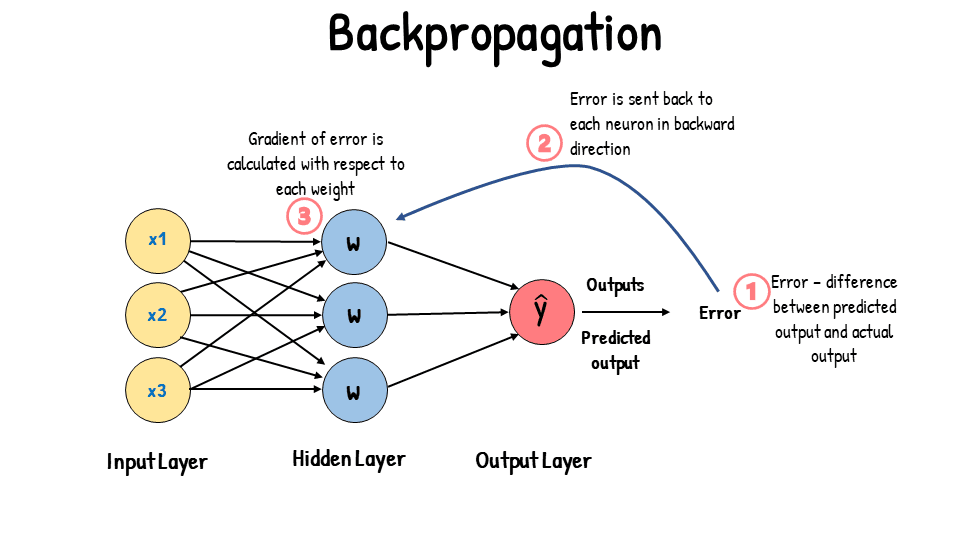
\includegraphics[width=1\textwidth]{chap2/figure/backprop.png}
    \caption{Intuitive representation of backpropagation \cite{botpenguin_backprop}.}
    \label{fig:back}
\end{figure}


\subsection{Convolutional Neural Networks}

The integration of prior knowledge into convolutional filters allows neural networks to leverage known properties of image data. In images, important information is often concentrated within local pixel neighborhoods, and similar visual patterns, such as edges or textures, can appear at different positions within the frame. Convolutional layers explicitly encode these assumptions in their architecture \cite{Li2020}. Each neuron connects only to a small, localized region of the input, reflecting the idea that nearby pixels are correlated. Moreover, the same set of weights (the convolutional kernel) is shared across all spatial locations, enforcing translation invariance and enabling the detection of identical features regardless of their position. This design reduces the number of trainable parameters, enhances generalization, and aligns with principles observed in biological visual systems.


Mathematically, the convolution operation between two functions $f(t)$ and $g(t)$ is defined as:
\begin{equation}
(f * g)(t) = \int_{-\infty}^{+\infty} f(\tau) g(t - \tau) d\tau
\end{equation}
where $(f * g)(t)$ is the result of convolving $f$ with $g$, and $g$ is commonly called the kernel or filter \cite{OShea2015}. In image processing, the kernel is a small matrix of weights that slides over the input tensor, computing local weighted sums to produce a feature map.

After the convolution operation, which the Figure \ref{fig:conv} describes, a non-linear activation function such as the \gls{relu} is typically applied to introduce non-linearity. To further reduce the dimensionality and retain the most salient features, pooling layers, such as max pooling, are used, which select the maximum value within a specified region of the feature map \cite{Li2020}. This combination of convolution, activation, and pooling enables convolutional neural networks to efficiently learn hierarchical representations from data.

\begin{figure}[ht]
    \centering
    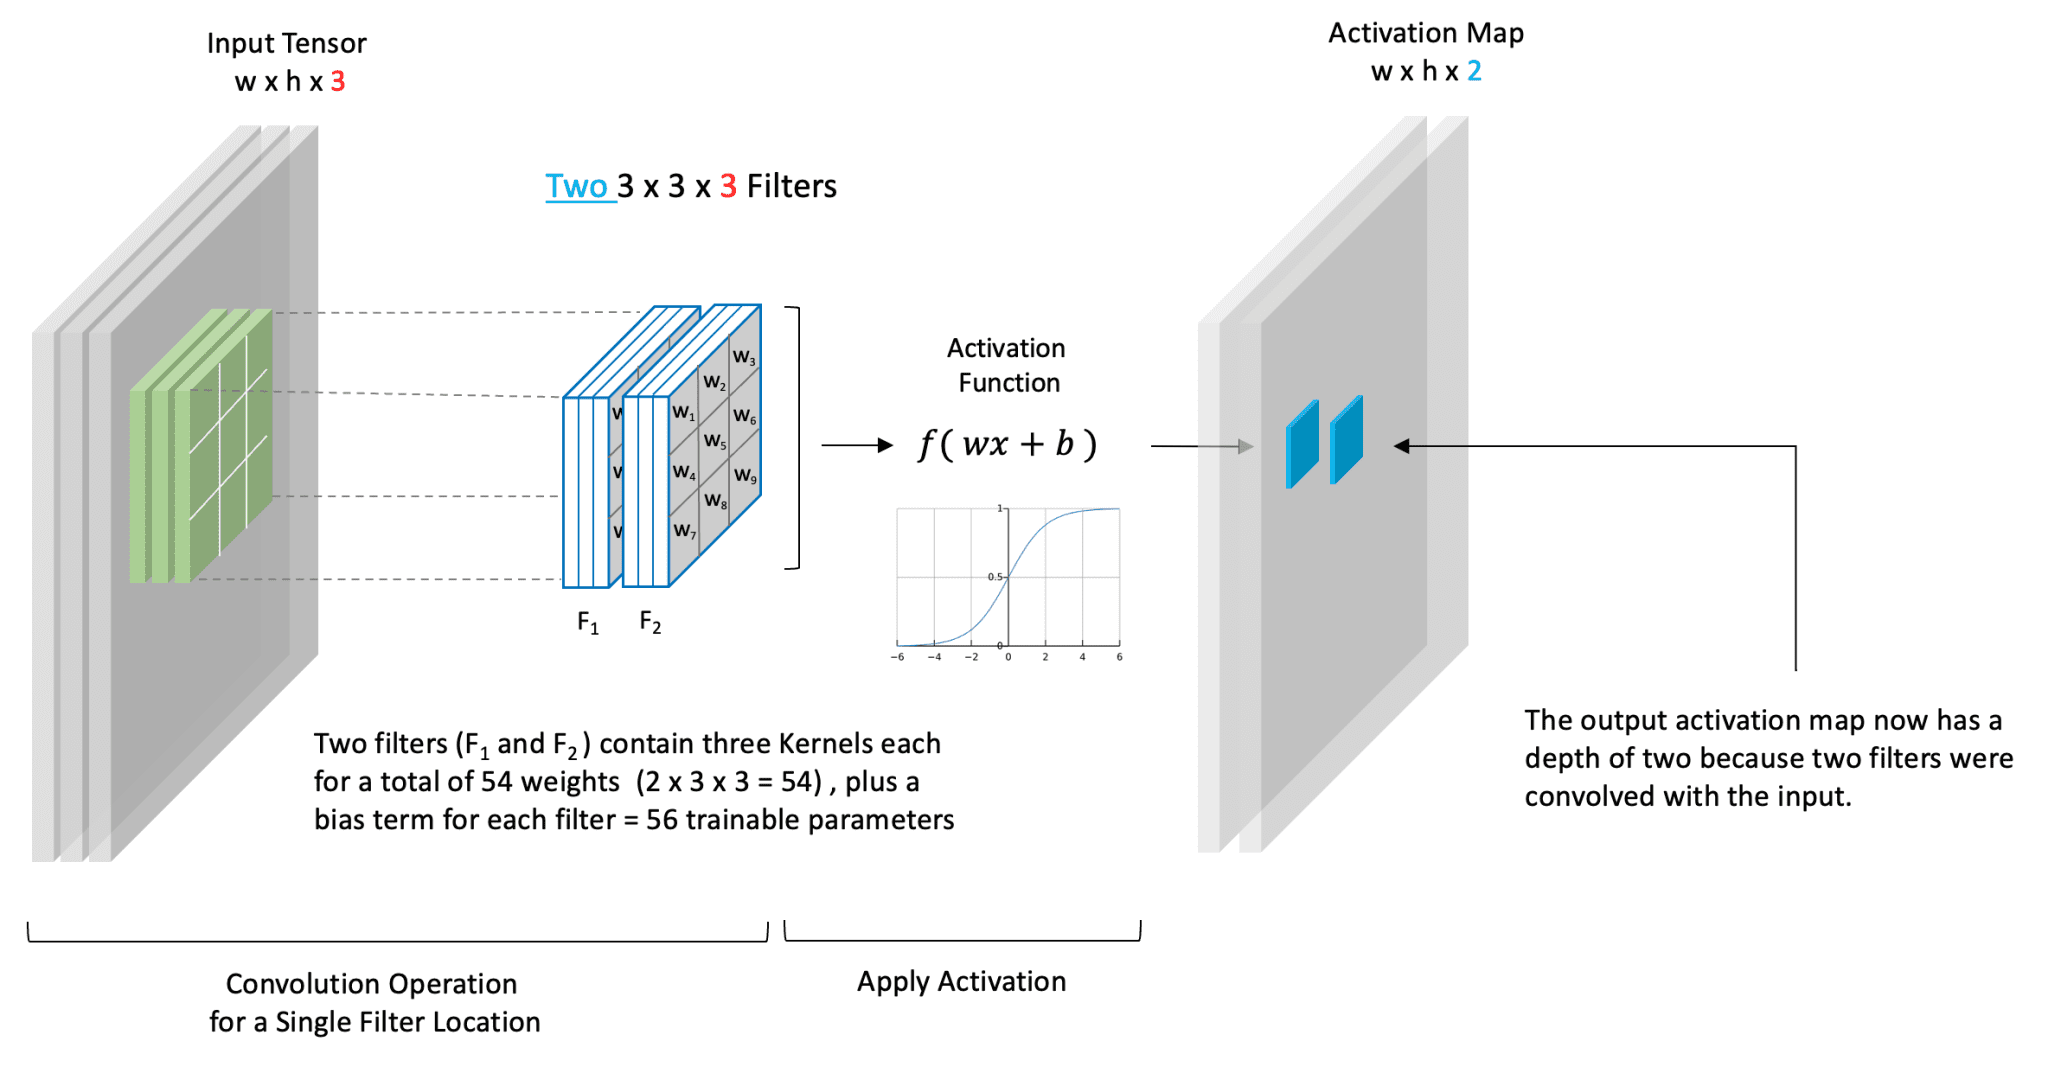
\includegraphics[width=1\textwidth]{chap2/figure/convolution.png}
    \caption{Representation of convolution \cite{learnopencv_cnn}.}
    \label{fig:conv}
\end{figure}


\subsection{Recurrent Neural Networks}

\glspl{rnn} are designed to model sequential data where the output at each time step depends not only on the current input but also on previous states. This is achieved by maintaining a hidden state that is updated recursively as new inputs are processed. The basic \gls{rnn} cell computes the hidden state $h_t$ at time $t$ using the following equation:
\begin{equation}
h_t = \tanh(W_x x_t + W_h h_{t-1})
\end{equation}
where $x_t$ is the input at time $t$, $W_x$ and $W_h$ are weight matrices, and $\tanh$ is a non-linear activation function \cite{Schmidt2019}. \glspl{rnn} are widely used for tasks such as language modeling, event prediction, and time series analysis.
The Figure \ref{fig:rnn} shows intuitively the difference between an RNN architecture and a Feed-Forward one.

\begin{figure}[ht]
    \centering
    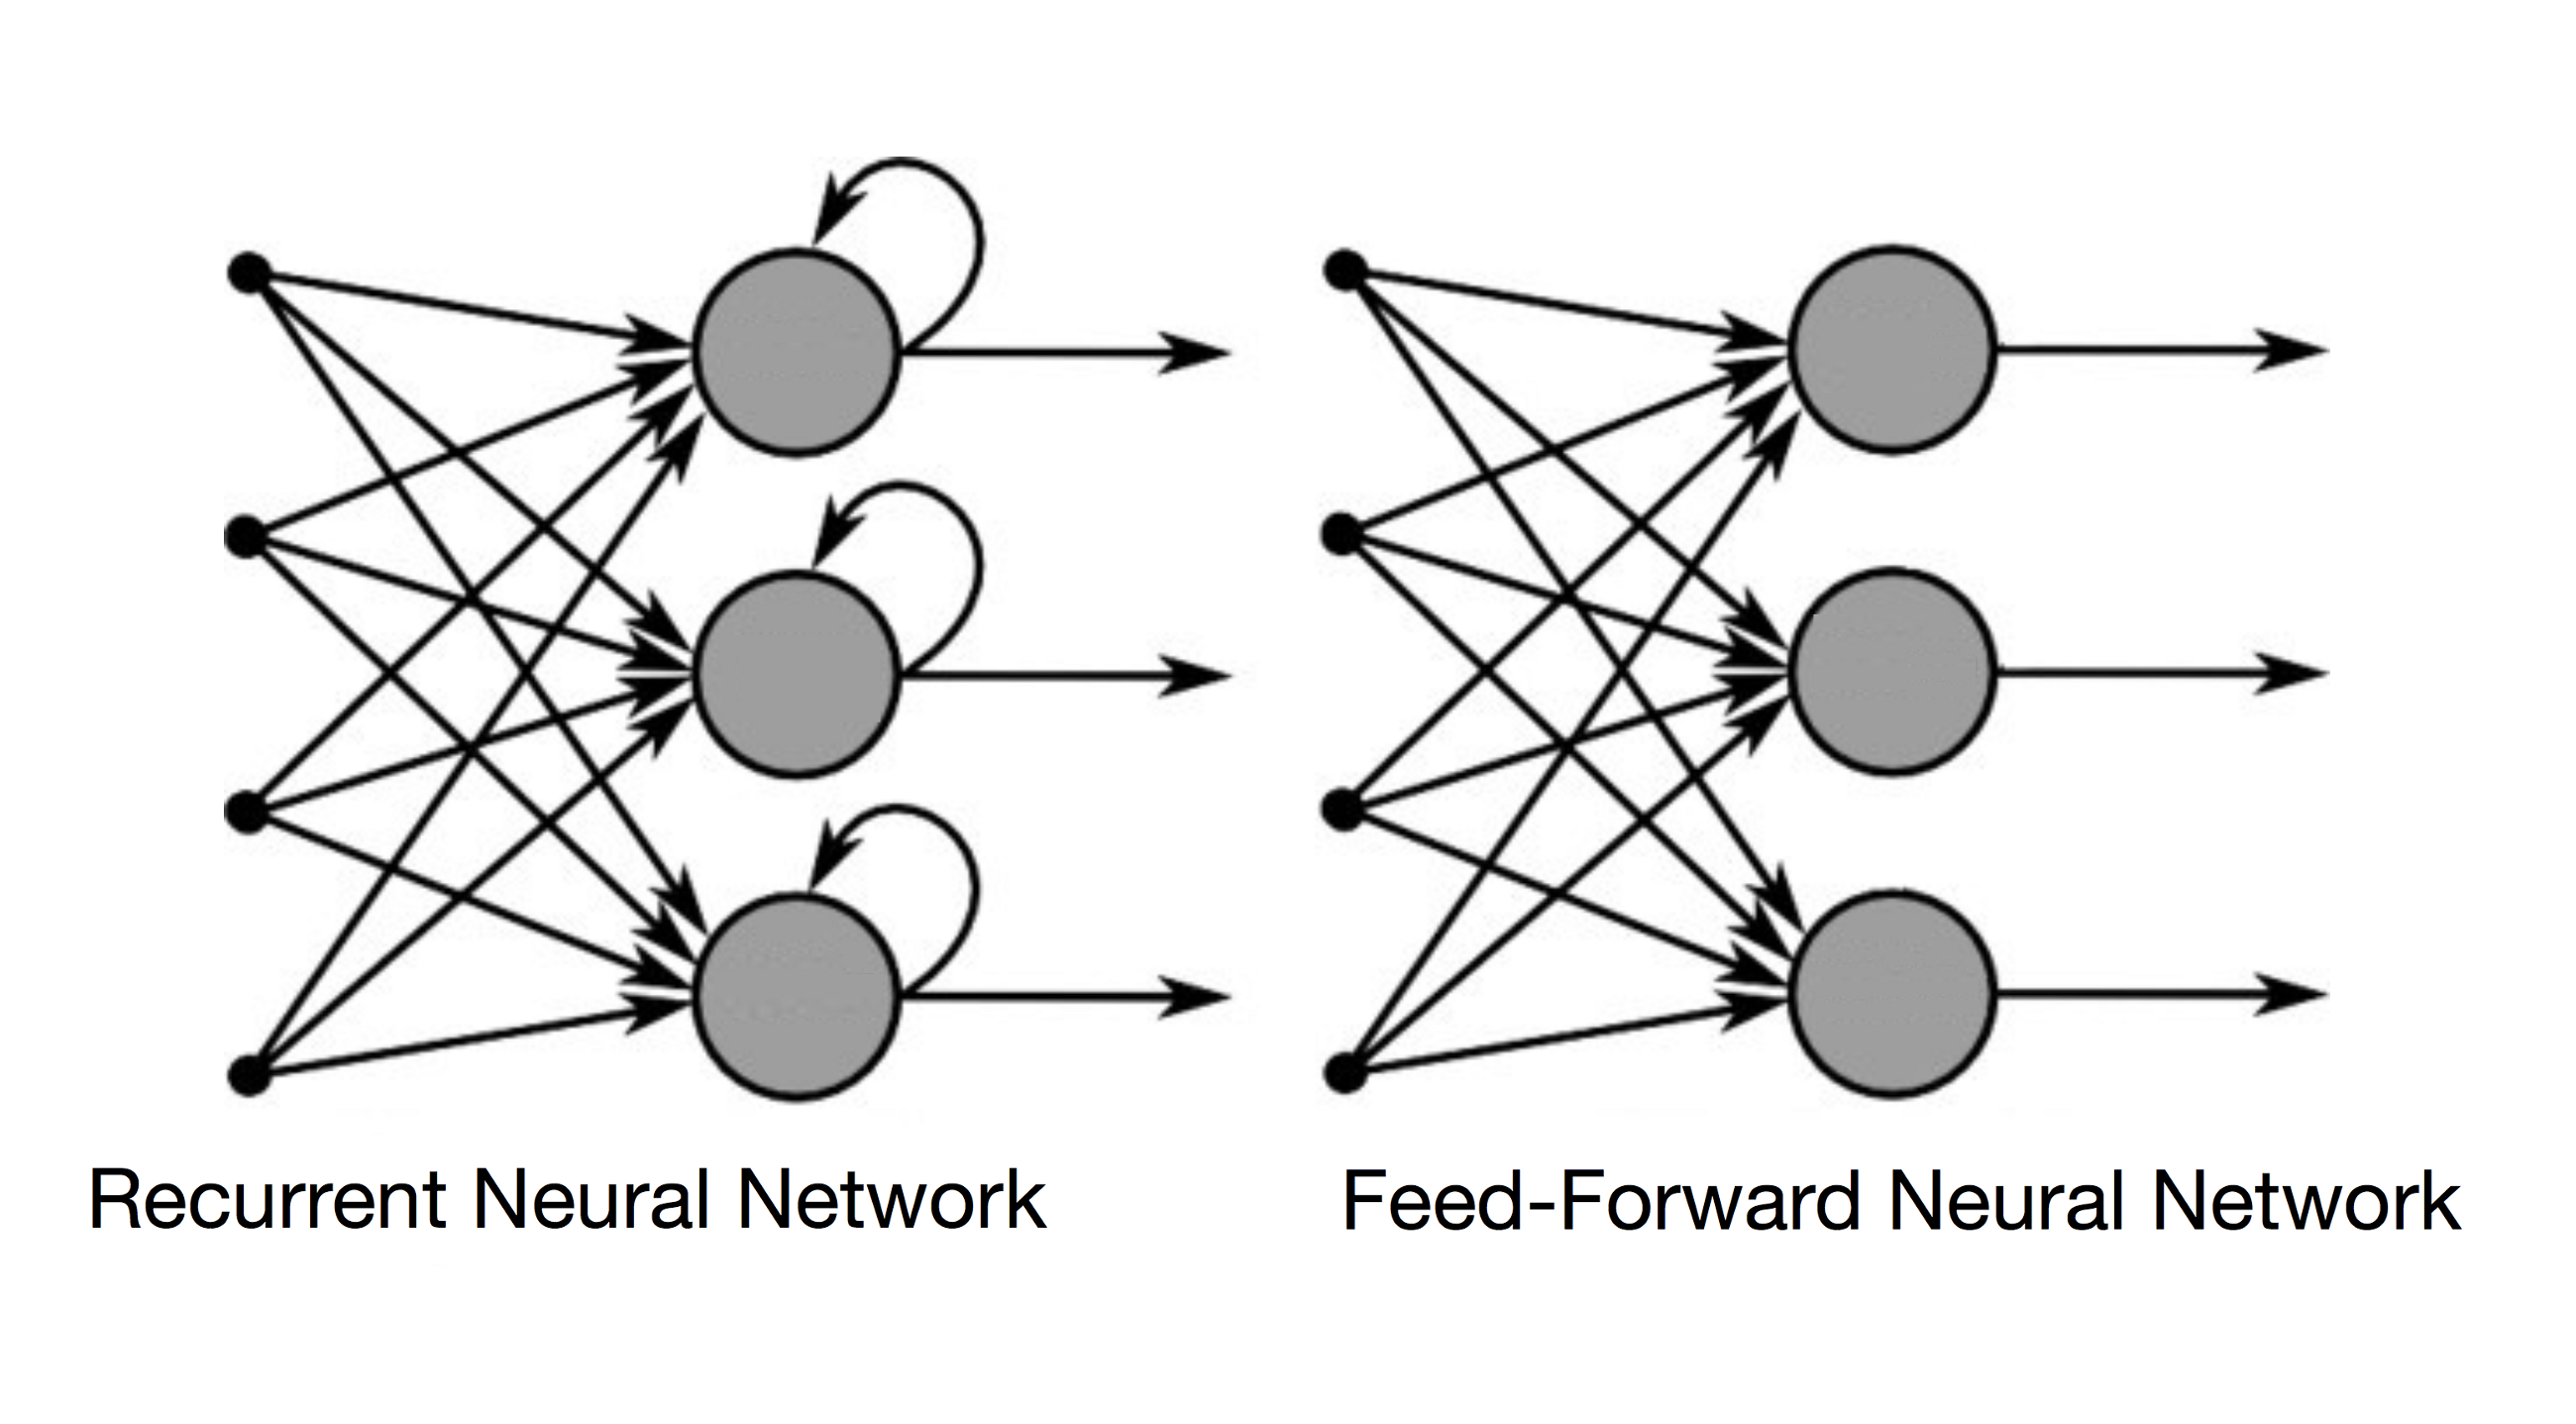
\includegraphics[width=1\textwidth]{chap2/figure/rnn.png}
    \caption{RNN vs Feed Forward Neural Network \cite{medium_rnn_classification}.}
    \label{fig:rnn}
\end{figure}


However, vanilla \glspl{rnn} often suffer from the vanishing and exploding gradient problems during training. The vanishing gradient problem occurs when gradients become exceedingly small, making it difficult for the network to learn long-term dependencies. Conversely, the exploding gradient problem arises when gradients grow uncontrollably, leading to unstable training. Gradient clipping can help mitigate exploding gradients, while architectural innovations such as Long Short-Term Memory (LSTM) and Gated Recurrent Unit (GRU) cells address vanishing gradients by introducing gating mechanisms that regulate information flow \cite{Salehinejad2018}.

LSTM cells enhance the memory capabilities of RNNs by maintaining both a hidden state $h_t$ and a cell state $c_t$. The gating system consists of input, forget, output, and gate gates, which are computed as follows:
\begin{align}
i_t &= \sigma(W_i [h_{t-1}, x_t]) \\
f_t &= \sigma(W_f [h_{t-1}, x_t]) \\
o_t &= \sigma(W_o [h_{t-1}, x_t]) \\
g_t &= \tanh(W_g [h_{t-1}, x_t])
\end{align}
The cell and hidden states are updated by:
\begin{align}
c_t &= f_t \ast c_{t-1} + i_t \ast g_t \\
h_t &= o_t \ast \tanh(c_t)
\end{align}
To update the cell state $c_t$ at time step $t$, the previous cell state $c_{t-1}$ is first modulated by the forget gate $f_t$, which determines the extent to which past information should be retained. Simultaneously, the input gate $i_t$ regulates how much new information, derived from the current input $x_t$, is incorporated into the cell state. This dual mechanism allows the LSTM to selectively preserve or overwrite information as needed.

The hidden state $h_t$ is then computed by applying the output gate $o_t$ to the transformed cell state, effectively controlling how much of the internal memory is exposed to the next layer or as output. This gating structure enables the LSTM to flexibly manage the flow of information across time steps.

A key reason why LSTMs mitigate the vanishing gradient problem is that, during backpropagation, the gradient with respect to the cell state is propagated primarily through element-wise multiplication by the forget gate $f_t$. This avoids repeated multiplication by weight matrices, which in traditional RNN can cause gradients to diminish exponentially. As a result, LSTMs are able to maintain and learn long-range dependencies, making them effective for modeling sequences with extended temporal structure \cite{Schmidt2019, Salehinejad2018, Lipton2015}.

